\chapter{算法设计}

\section{问题描述}
对于给定一个以自然句子表示的即席查询$s$,共包含$l$个单词$\{w_1,w_2,\ldots,\\w_l\}$,本文研究的目标是建立一个
视频检索系统,即从$n$个未被标注的视频集$\mathcal{V}=\{v_1,v_2,\ldots,v_n\}$中搜索出与该查询语义相关的视频。问题的关键是构建
一个跨模态的相似度函数$cms(s,v) \in \mathbb{R}$,使得相关的句子视频对$(s,v^+)$的相似度比不相关的句子视频对$(s,v^-)$
更大。相应地,根据这个相似度对视频集合$\mathcal{V}$中的所有视频降序排序,则在查询结果中相关的视频$v^+$会排在不相关的视频$v^-$的视频前,从而检索系统返回排序靠前的视频。而$s$和$v$的相似度$cms(s,v)$计算需要将$s$和$v$在公共的跨模态空间进行合适的向量化表示,在得到视频在公共空间的向量化表示前需要先用深度卷积网络来提取视频的特征,而句子则需要用文本编码器如bow得到句子的向量。设$e_t$是一个可以将句子编码成一个$d_t$维向量的文本编码器,即$e_t(s) \in \mathbb{R}^{d_t}$,如果有$k$个文本编码器$\{e_{t,1},\ldots,e_{t,k}\}$同时对查询句子进行编码,则会得到$k$个不同维度$\{d_{t,1},\ldots,d_{t,k}\}$的句子向量。然后需要对这些查询句子向量和视频特征投影到公共的跨模态空间,
设$\mathbf{s}$和$\mathbf{v}$是查询句子与视频
在公共空间的向量化表示,则跨模态的相似度由余弦相似度得到:
\begin{equation}
    \label{eq:cosine-sim}
    \begin{aligned}
        cms(s,v) := \frac{\mathbf{s}^T\mathbf{v}}{\left\| \mathbf{s} \right\| \cdot \left\| \mathbf{v} \right\|}
    \end{aligned}
\end{equation}

本文着眼于查询表示学习,即由查询$s$获得获得$k$个文本编码向量$\{e_{t,1}(s),\\ \ldots,e_{t,k}(s)\}$,并有效地利用这些文本编码器,从而得到查询$s$在公共空间的向量表示$\mathbf{s}$,而视频可以像之前的工作一样由深度卷积网络得到
的特征或者概念向量表示。

\section{句子编码器}
本文是建立在Word2VisualVec(W2VV)~\cite{dong2018predicting}模型的基础上,W2VV模型原本是用在图像描述或者视频描述的检索任务上,概念模型图如\ref{fig:base-w2vv}所示,该模型共包含两个子网络,即一个句子编码网络,把一个句子向量化和一个转换网络,将句子向量转换到视觉特征空间中。W2VV模型的句子编码网络由三个文本编码器并行对句子进行向量化,即bag-of-words (bow),word2vec (w2v)和Gated Recurrent Unit (GRU),最后使用拼接的方式融合由这三种编码器得到句子向量,而转换网络是由多层全连接层组成的多层感知机,他们的训练目标是最小化在视觉空间中的句子向量和视频向量之间的平方误差。考虑到W2VV模型使用的GRU编码器只取了最后时刻的输出向量,并且只通过简单地拼接这三种向量,作为句子的向量表示不是一种最优的方法,训练时只考虑减小正样本视频-文本对的欧式距离,并没有增大考虑负样本视频-文本对的距离,而对于一个新来的查询句子,可能会与负样本视频的距离同样很小,因此这也不是一个最优的训练目标。
\begin{figure*}[tbh!]
    \centering
    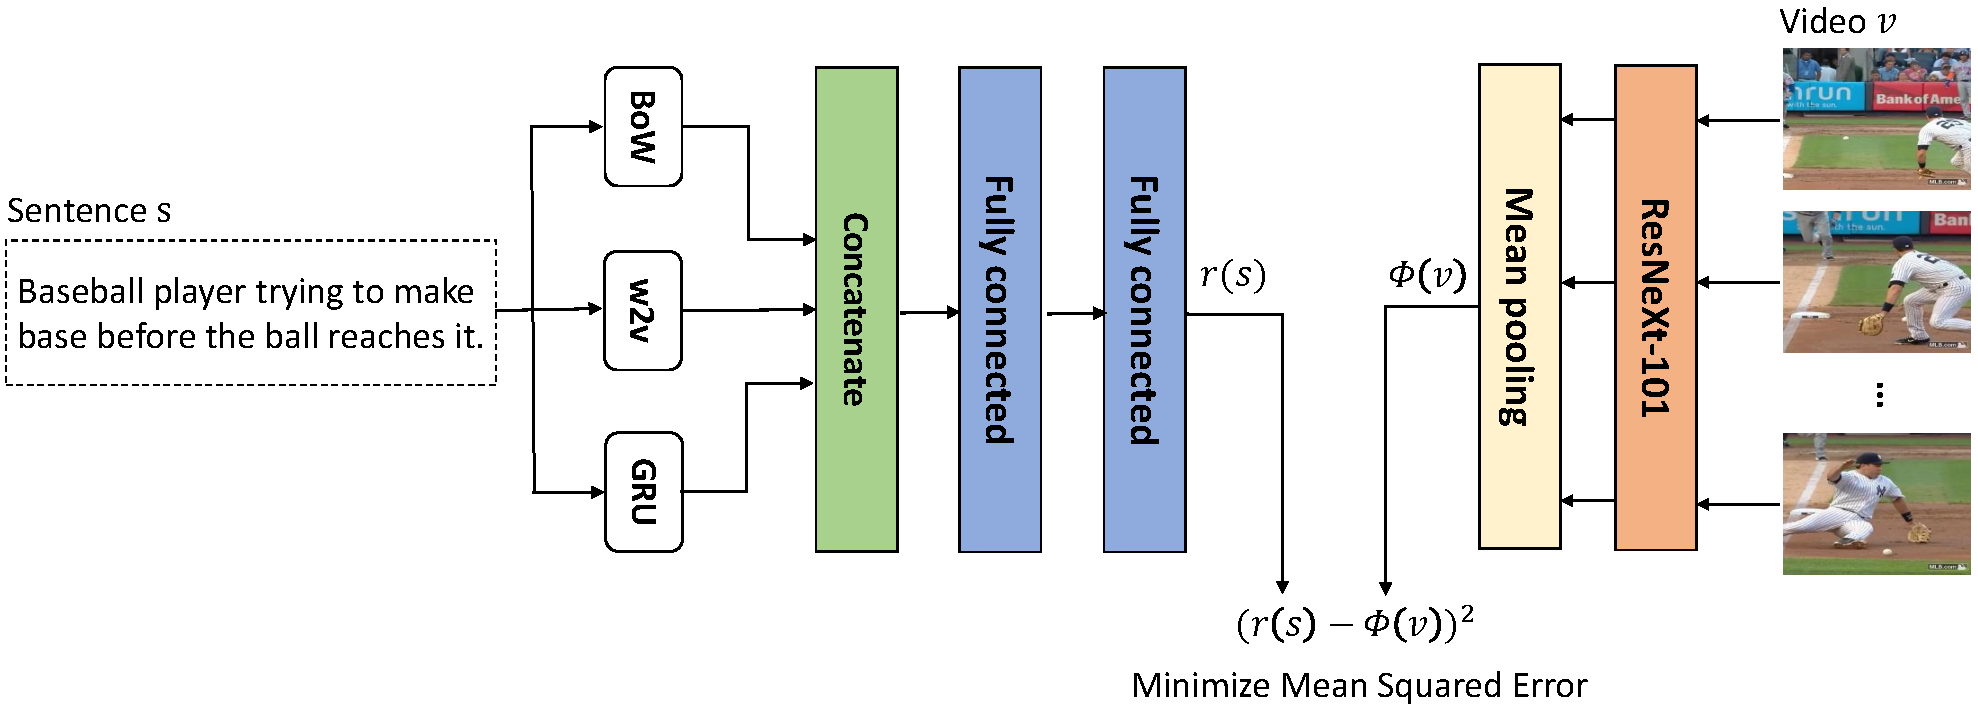
\includegraphics[width=\linewidth]{figures/w2vv-model}
    \caption[Dong等人~\cite{dong2018predicting}提出的W2VV模型的概念图]{\textbf{W2VV模型概念图,来自~\cite{li2017multi}。该模型包含两个子网络,第一个是句子编码网络,句子同时被三种编码器进行向量化编码,即bag-of-words (bow),word2vec (w2v),和Gated Recurrent Unit (GRU),第二个是转换网络,是由两层全连接组成的感知机,将拼接的三种句子编码向量投影到视觉特征空间中,并在训练时使用正样本的句子-视频来优化平均平方误差的目标函数。}}
    \label{fig:base-w2vv}
\end{figure*}

鉴于此,本文基于W2VV模型使用一个更优的编码策略和一个更优的目标函数用于训练,即对于GRU,本文采用平均池化的方法处理其所有的隐藏状态输出表示该文本的GRU输出,并且使用improved triplet ranking loss (ITRL)~\cite{faghri2017vse++}作为训练目标,该训练目标在训练时同时增大正样本视频-文本对的相似度并且减小负样本视频-文本对的相似度,为了方便,本文将此模型命名为W2VV++,模型结构图如图~\ref{fig:w2vv++}所示。而对于不同的编码器之间的融合,本文在W2VV++的基础上继续研究多子空间融合的方法,即为不同的编码器独立构建公共的跨模态空间,最后在同一个模型内融合这些公共空间得到最终的跨模态相似度计算,本文将这种融合模型称为Sentence Encoder Assembly (SEA),模型结构图如图~\ref{fig:sea}。接下来,本文将介绍本文使用的三种文本编码器,即bag-of-words (bow),word2vec (w2v)和Gated Recurrent Unit (GRU)。

\begin{figure*}[tbh!]
    \centering
    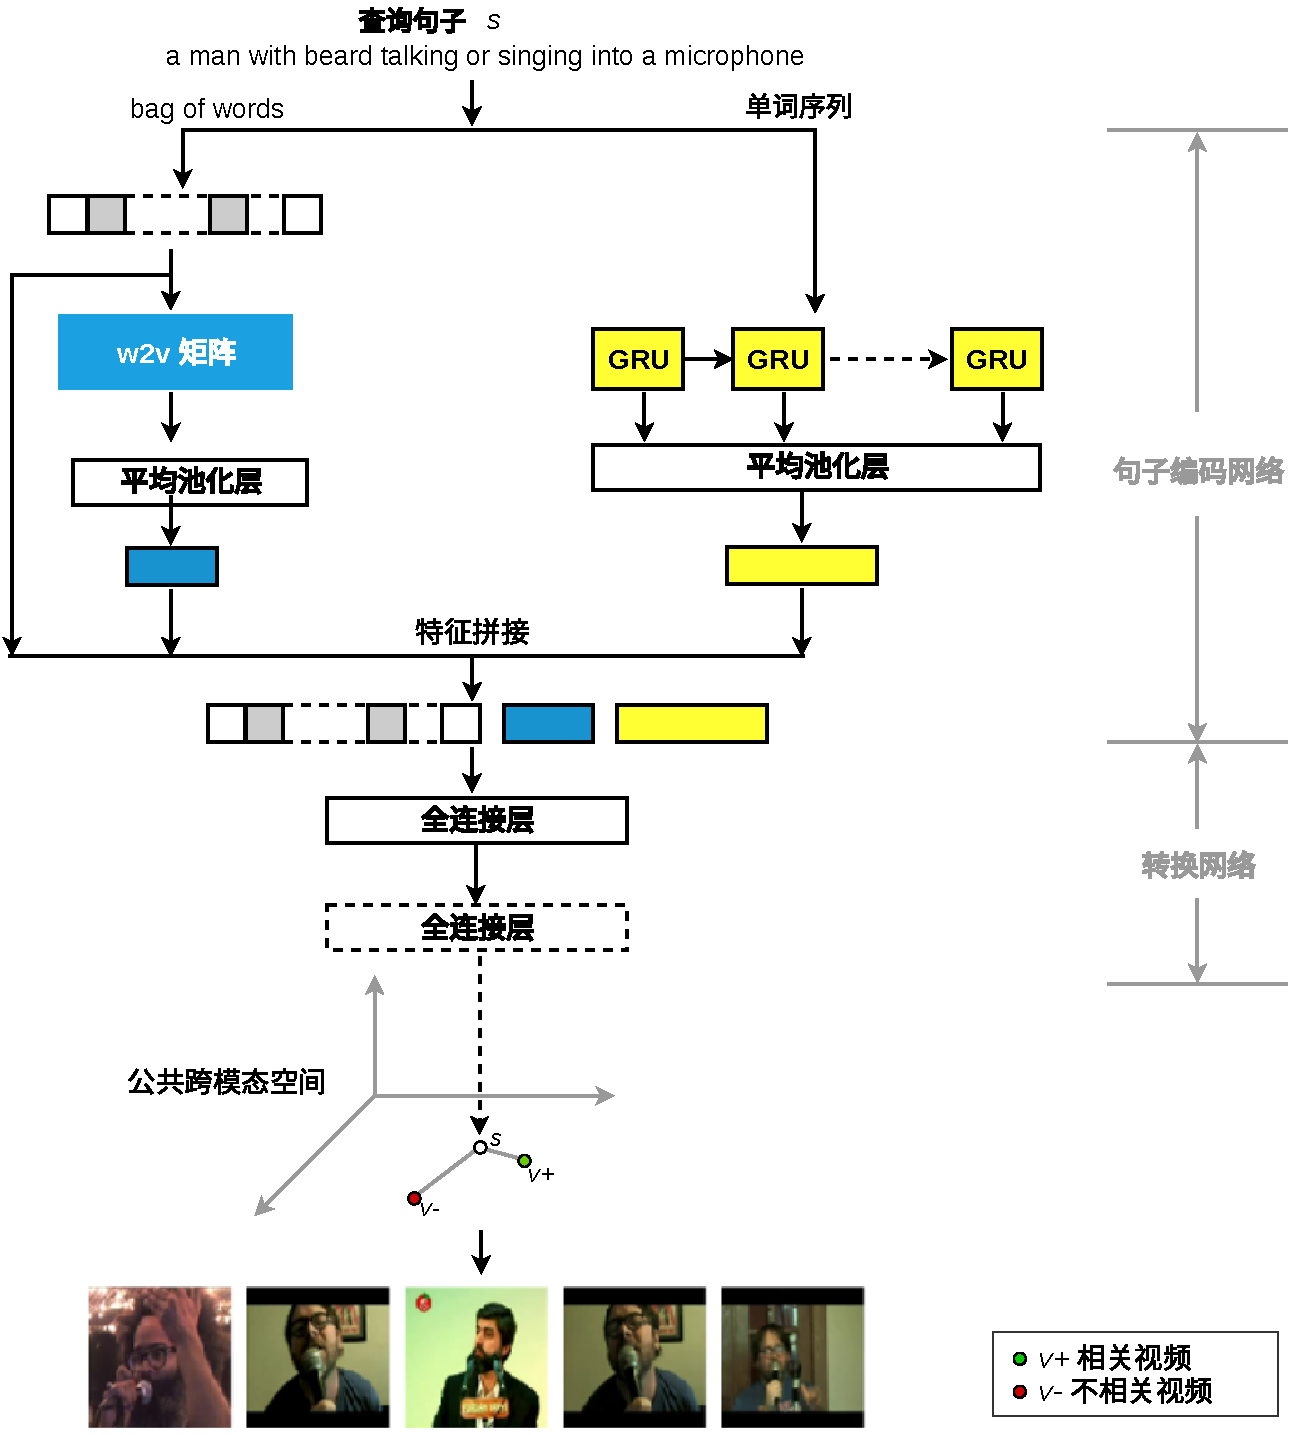
\includegraphics[width=\linewidth]{figures/w2vv++v2}
    \caption[即席视频检索模型W2VV++概念图]{\textbf{即席视频检索模型W2VV++概念图。该模型基于W2VV模型~\cite{dong2018predicting}进行改进,使用平均池化的操作利用了GRU编码的所有时刻的隐藏状态输出。为了利用充足的负样本句子-视频对,W2VV++的训练优化目标是improved triplet ranking loss (ITRL)~\cite{faghri2017vse++},而不是W2VV模型的只考虑了正样本的句子-视频对的平均平方误差。}}
    \label{fig:w2vv++}
\end{figure*}

\begin{figure*}[tbh!]
    \centering
    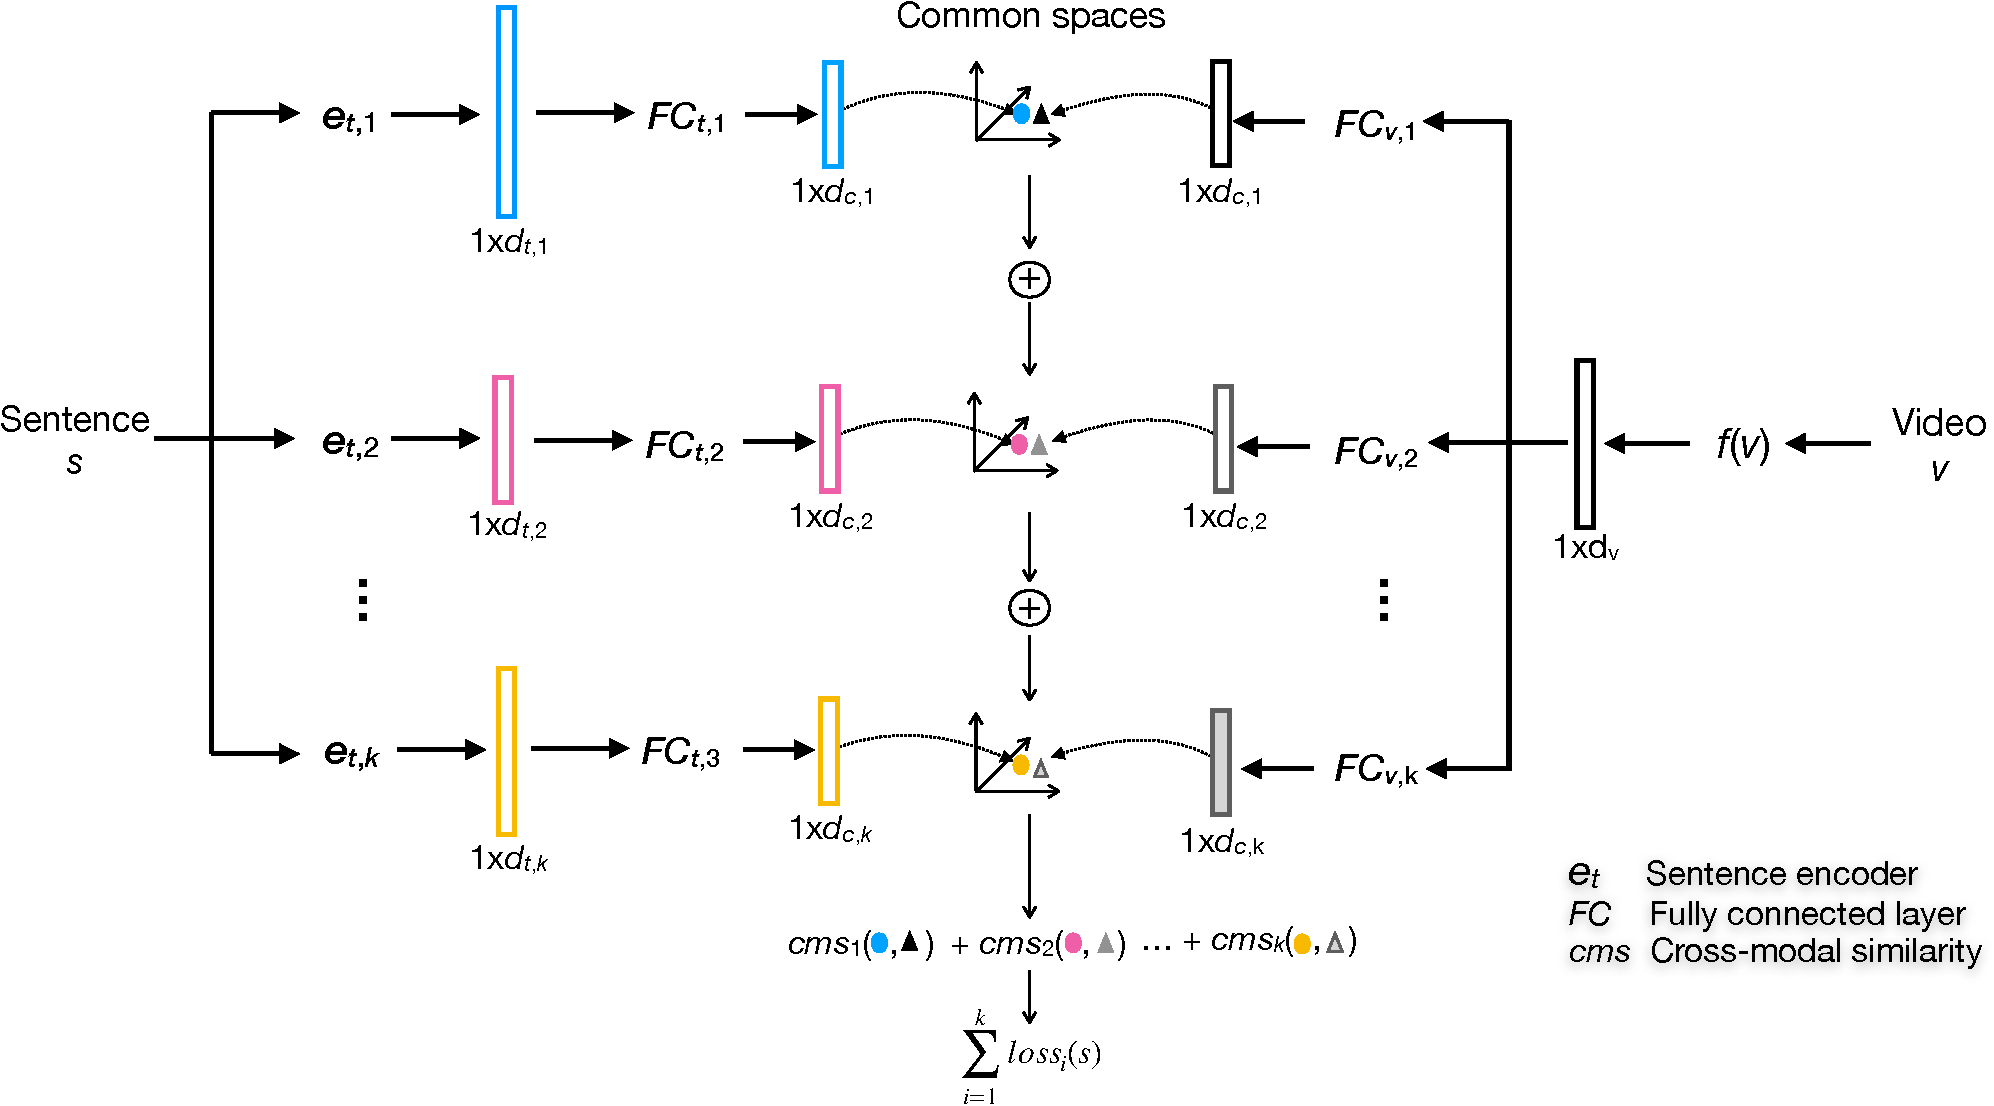
\includegraphics[width=\linewidth]{figures/sea}
    \caption[即席视频检索模型SEA概念图]{\textbf{即席视频检索模型Sentence Encoder Ensembles (SEA)概念图。该模型为每个句子编码器构建独立的公共跨模态空间,即每个句子编码器输出的句子向量都经过转换网络投影到独立的公共空间中,而最终的句子与视频的相似度由句子与视频在所有公共空间中计算的相似度取平均得到,SEA采用多空间多目标函数的训练策略,即为每个公共空间独立地计算和优化目标函数ITRL。}}
    \label{fig:sea}
\end{figure*}

\textbf{bow}:对于给定的一个句子$s$,对于bow编码技术,句子$s$的向量可以由如下式子得到:
\begin{equation}
    \label{eq:bow}
    \begin{aligned}
        e_{bow}(s) := (c(w_1,s),c(w_2,s),\cdots,c(w_m,s))
    \end{aligned}
\end{equation}
其中,$c(w,s)$计算特定单词$w$在句子$s$中出现的次数,$m$表示给定词典的单词数量,本文使用的词典由在训练数据中出现不少于5次
的单词组成,并且根据NLTK去掉其中的停用词。由于给定的词典是由训练集确定的,通常超过一万维,而AVS查询句子通常是比较短,平均长度不超过10个单词,因此bow编码的向量$e_{bow}(s)$是一个非常高维但稀疏的向量。

w2v:与bow编码器不同,w2v模型~\cite{mikolov2013efficient}通过用一个很大的文本语料训练一个两层的神经网络来产生单词的稠密的语义向量。因为w2v模型的训练目标是重建句子的上下文信息,因此不需要对训练数据进行人工标注,因此可以很容易地对成千上万的单词进行编码。对于一个给定的预训练w2v模型,设$w2v(w_i)$是可以得到句子$s$的第$i$个单词的词向量,本文通过对$s$中所有单词的w2v向量进行平均池化操作得到句子的向量,具体计算如下:
\begin{equation}
    \label{eq:w2v}
    \begin{aligned}
        e_{w2v}(s) := \frac{1}{l}\sum^l_{i=1}w2v(w_i)
    \end{aligned}
\end{equation}
本文使用的是一个500维的使用3000万张Flickr图像的英文标签训练的w2v模型~\cite{dong2018predicting},共支持超过170万个常见的单词向量化。

GRU:和W2VV相似,本文同样使用Gated recurrent unit (GRU)~\cite{cho2014learning}作为序列模型对句子进行建模。GRU在特定的$t$时刻的输入
是句子中第$t$个单词的词嵌入向量,设为$e(w_t)$,该向量是从一个词嵌入矩阵$W_e$中对应的单词的词嵌入向量得到的,并作为网络的可学习参数和GRU一同进行端到端训练。而当前时刻GRU的输出,设为$h_t$是通过联合当前词嵌入向量$e(w_t)$和前一时刻GRU的输出向量$h_{t-1}$由如下式子得到:
\begin{equation}
    \label{eq:gru}
    \begin{aligned}
        & z_t = \sigma_g(W_z e(w_t) + U_z h_{t-1} + b_z), \\
        & r_t = \sigma_g(W_r e(w_t) + U_r h_{t-1} + b_r), \\
        & \widetilde{h_t} = \sigma_h(W_h e(w_t) + U_h (r_t \circ h_{t-1}) + b_h), \\
        & h_t = (1-z_t) \circ h_{t-1} + z_t \circ \widetilde{h_t},
    \end{aligned}
\end{equation}
其中$z_t$ 和$r_t$表示在$t$时刻的更新门向量和重置门向量,$W$,$U$和$b$表示门的仿射转换参数,每个门输出前带有一个特定的激活函数,其中
$\sigma_g$表示sigmoid函数,$\sigma_h$表示双曲正切函数,操作$\circ$为两个向量的哈达玛积,即逐元素相乘。

对于基于GRU的句子编码,W2VV只取最后时刻的输出向量,即$h_l$,而本文通过对所有时刻的输出向量进行平均池化操作,考虑了所有的中间时刻的输出状态,即:
\begin{equation}
    \label{eq:gru-mean}
    \begin{aligned}
        e_{gru}(s) := \frac{1}{l}\sum^l_{i=1}h_i
    \end{aligned}
\end{equation}
对于GRU词典,与bow词典类似,但是GRU词典还包含停用词,因为它们在自然语句中是含有意义的上下文信息。

W2VV++模型:如图~\ref{fig:w2vv++}所示,W2VV++模型通过使用拼接的方式融合这三种编码器输出的向量,设$e_{ms}(s)=[e_{bow}(s);e_{w2v}(s);e_{gru}(s)]$,其中$[;;]$表示向量拼接操作,向量$e_{ms}(s)$通过转换网络投影到与视频的公共跨模态空间,在该公共空间计算查询句子与视频的相似度$cms(s,v)$。

SEA模型:如图~\ref{fig:sea}所示,SEA模型通过为每个编码器构建一个独立的公共跨模态空间,在每个公共空间单独计算查询句子与视频的相似度$cms_i(s)$,$i$表示在第$i$个公共空间,并使用相加的方式融合各个空间中的相似度作为最终的查询句子与视频的相似度,即$cms_1(s,v)+cms_2(s,v)+cms_3(s,v)$。

%对于多种编码方式(bow, w2v, GRU)对句子进行编码,本文使用两种策略对这些编码方式进行融合,即:
%\begin{itemize}
%    \item W2VV++:使用与W2VV相同的方式,即向量拼接融合,即$\bm{\mathbf{ms}}(s)=[\bm{\mathbf{bow}}(s);\bm{\mathbf{w2v}}(s);\bm{\mathbf{gru}}(s)]$。本文将这种方式的模型称为W2VV++。
%
%    \item TEE:三种编码方式互相独立,分别与视频向量。本文将这种方式的模型称为text encoding ensemble(TEE)。
%\end{itemize}

\section{视频特征表示}
正如前文所言,本文研究关注于查询表示学习,因此,对于视频的表示,本文简单地使用当前最好的深度卷积网络通过过采样的方式对帧图像提取视觉特征,
并且使用平均池化的操作对帧图像进行聚合操作从而获得视频的特征表示,如图\ref{fig:video-cnn-feat}所示。

\begin{figure*}[tbh!]
    \centering
    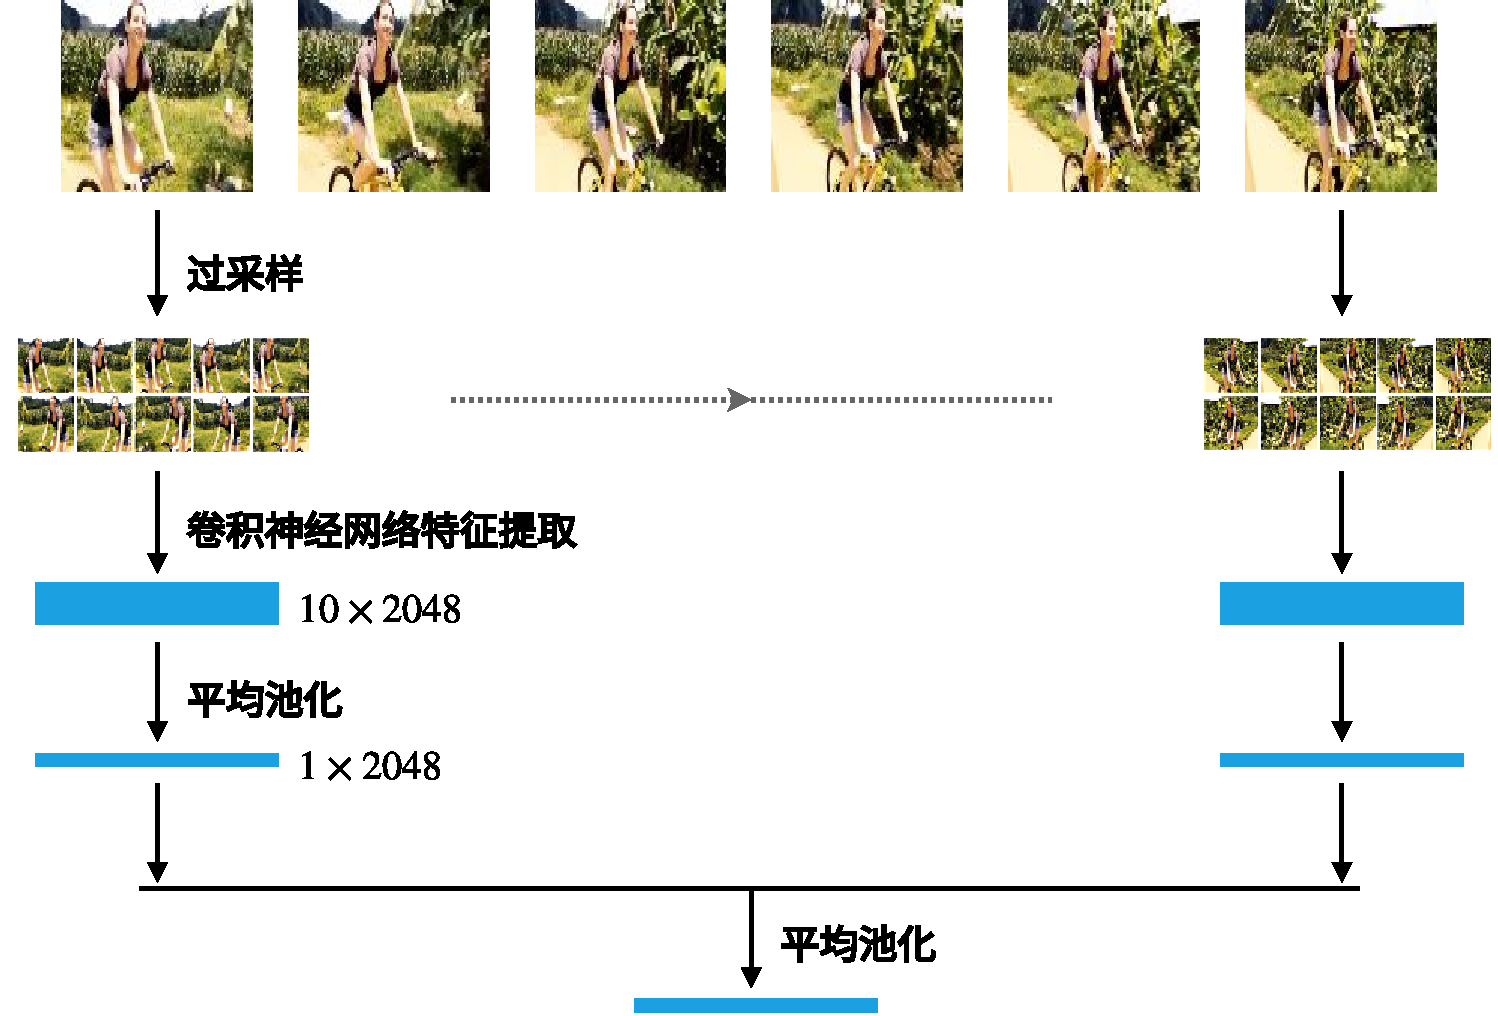
\includegraphics[width=\linewidth]{figures/video-cnn-feat}
    \caption[视频特征提取示例图]{\textbf{视频特征提取示例图。本文使用在图像识别上预训练的深度卷积网络以过采样的方式提取视频的帧图像的特征,并用平均池化的操作聚合帧图像特征从而得到视频级特征。}}
    \label{fig:video-cnn-feat}
\end{figure*}

本文使用两个深度卷积网络模型进行视频的特征提取:
ResNeXt-101~\cite{xie2017aggregated}和ResNet-152~\cite{he2016deep}。对于每个模型,本文选择模型的分类层输出作为特征,维度为2048维。
对于给定一个视频,本文以0.5秒为间隔对视频的帧图像进行均匀采样。每张采样的图像的大小调整为$256\times256$,然后以$224\times224$大小
的窗口对该图像与其水平翻转得到的图像的四个角和中央进行裁剪,得到该图像的10张子图,这10张子图分别经过卷积网络提取特征并且进行
平均池化操作,得到该图像的特征表示。相应地,2048维的视频特征由帧图像特征进行平均池化得到。为了方便表示,本文将使用$ResNeXt$和$ResNet$
表示经过这两种卷积网络得到的视频特征,$ResNeXt$-$ResNet$表示这两种特征进行拼接得到的4096维的视频特征,设视频$v$的深度卷积特征向量为$f(v) \in \mathbb{R}^{d_v}$。

原则上,本文的模型可以使用任何的视频特征表示,包括概念特征向量~\cite{markatopoulou2017query,lu2016event,merler2012semantic}和3D卷积网络特征~\cite{mithun2018learning}。

\section{转换网络}
由前文可在,计算查询句子$s$和视频$v$的跨模态相似度$cms(s,v)$需要将$s$和$v$在公共的跨模态空间进行向量化表示,则在得到句子的编码向量表示和视频的特征表示后,关键一步是将这两个模态的向量化表示转换到维度相同向量。转换网络以上一层的编码网络输出作为输入,并将输入的向量转换成另一个维度的向量。

%和转换网络用于将之前的网络输出进行非线性仿射变换,即对于W2VV++模型,将$\bm{\mathbf{ms}}(s)$进行转换,对于TEE模型,分别对$\bm{\mathbf{bow}}(s)$,$\bm{\mathbf{w2v}}(s)$和$\bm{\mathbf{gru}}(s)$进行转换,
%把文本编码得到的向量转换到一个公共空间,得到向量$\bm{\mathbf{s}}$,使得句子与视频的相关性可以由公式\ref{eq:cosine-sim}进行计算。
本文使用$n$层全连接层实现该转换网络,设上一层网络的输出向量,即转换网络的输入向量为$g$,设$g \in \mathbb{R}^{d_1}$,则第一层全连接层
的输出向量$\bm{\mathbf{fc^1}}(s)$由作用在向量$g$的仿射变换得到,即:
\begin{equation}
    \label{eq:fc-1}
    \begin{aligned}
        \bm{\mathbf{fc}}^1(s) = \sigma(A_1 g + b_1)
    \end{aligned}
\end{equation}
其中$A_1 \in \mathbb{R}^{d_2 \times d_1}$和$b_1 \in \mathbb{R}^{d_2}$分别是全连接层的权重和偏移,$\sigma$是增强网络非线性的激活函数,本文默认的激活函数是双曲正切函数$tanh$。转换网络的剩余的全连接层计算如下公式:
\begin{equation}
    \label{eq:fc-k}
    \begin{aligned}
        \bm{\mathbf{fc}}^i(s) = \sigma(A_i\bm{\mathbf{fc}}^{i-1}(s) + b_i), i=2,...,n.
    \end{aligned}
\end{equation}

%本文的句子编码网络和转换网络是端到端地进行训练的,把网络的所有可学习的参数$\{W_z,U_z,b_z,W_r,U_r,b_r,W_h,U_h,b_h,W_e,A_1,b_1,\cdots,A_k,b_k\}$表示成$\theta$,相应地,相似度函数参数表示为$cms(s,v;\theta)$。

W2VV++模型:对于该模型,文本端的编码器的输出向量为$e_{ms}(s) \in \mathbb{R}^{d_t}$,因此文本端的转换网络的输入是$e_{ms}(s)$,设文本端的转换函数为$\bm{\mathbf{fc}}_t^n(s)$,则文本端的转换网络输出为$\mathbf{s} = \bm{\mathbf{fc}}_t^n(s)$,$\mathbf{s} \in \mathbb{R}^{d_c}$,对于视频端,设视频端的转换函数为$\bm{\mathbf{fc}}_v^n(v)$,则视频端的转换网络的输入是视频的深度卷积特征向量$f(v) \in \mathbb{R}^{d_v}$,转换网络的输出是$\mathbf{v} = \bm{\mathbf{fc}}_v^n(v)$,$\mathbf{v} \in \mathbb{R}^{d_c}$。因此在公共的跨模态空间,查询句子与视频的相似度可以由公式\ref{eq:cosine-sim}计算得到。

SEA模型:对于该模型,文本端的编码器输出向量分别为$e_{bow}(s) \in \mathbb{R}^{d_{t,1}}$,$e_{w2v}(s) \in \mathbb{R}^{d_{t,2}}$和$e_{gru}(s) \in \mathbb{R}^{d_{t,3}}$,如图~\ref{fig:sea}所示,该模型为每个文本编码器构建独立的公共跨模态空间,即每个编码器输出的向量都经过一个独立的转换网络,分别设为$\bm{\mathbf{fc}}_{t,1}^n(s)$,$\bm{\mathbf{fc}}_{t,2}^n(s)$,$\bm{\mathbf{fc}}_{t,3}^n(s)$,则文本端的转换网络输出分别为$\mathbf{s}_1 = \bm{\mathbf{fc}}_{t,1}^n(s)$,$\mathbf{s}_2 = \bm{\mathbf{fc}}_{t,2}^n(s)$,$\mathbf{s}_3 = \bm{\mathbf{fc}}_{t,3}^n(s)$,$\mathbf{s}_1 \in \mathbb{R}^{d_{c,1}}$,$\mathbf{s}_2 \in \mathbb{R}^{d_{c,2}}$,$\mathbf{s}_3 \in \mathbb{R}^{d_{c,3}}$。同样在视频端也有三个独立的转换网络,分别将视频特征$f(v)$转换到三个公共空间中,设三个转换网络分别为$\bm{\mathbf{fc}}_{v,1}^n(v)$,$\bm{\mathbf{fc}}_{v,2}^n(v)$,$\bm{\mathbf{fc}}_{v,3}^n(v)$,这三个视频端的转换网络的输入都是视频特征$f(v)$,而输出分别是为$\mathbf{s}_1 = \bm{\mathbf{fc}}_{v,1}^n(v)$,$\mathbf{v}_2 = \bm{\mathbf{fc}}_{v,2}^n(v)$,$\mathbf{v}_3 = \bm{\mathbf{fc}}_{v,3}^n(v)$,$\mathbf{v}_1 \in \mathbb{R}^{d_{c,1}}$,$\mathbf{v}_2 \in \mathbb{R}^{d_{c,2}}$,$\mathbf{v}_3 \in \mathbb{R}^{d_{c,3}}$。查询句子与视频的相似度由三个公共空间的句子-视频相似度的平均得到,即$cms(s,v) := \frac{1}{3}(cms_1(s,v)+cms_2(s,v)+cms_3(s,v))$:

\begin{equation}
    \label{eq:cosine-sim-3}
    \begin{aligned}
        cms_1(s,v)+cms_2(s,v)+cms_3(s,v) := \\
        \frac{\mathbf{s_1}^T\mathbf{v_1}}{\left\| \mathbf{s_1} \right\| \cdot \left\| \mathbf{v_1} \right\|}+\frac{\mathbf{s_2}^T\mathbf{v_2}}{\left\| \mathbf{s_2} \right\| \cdot \left\| \mathbf{v_2} \right\|}+\frac{\mathbf{s_3}^T\mathbf{v_3}}{\left\| \mathbf{s_3} \right\| \cdot \left\| \mathbf{v_3} \right\|}
    \end{aligned}
\end{equation}

\section{目标函数}
与W2VV模型的训练目标是最小化平均欧平方误差不同,本文使用改进的三元组排序损失函数(improved triplet ranking loss,ITRL),这个目标函数原本在Faghri等人在文献~\cite{faghri2017vse++}提出用在图像-文本的相互检索上,但是也被在基于文本的视频检索的一些工作上被证明了是有效的~\cite{mithun2018learning,dong2019dual,liu2019use,wu2019hybrid,li2019w2vv++}。经典的三元组排序损失函数从训练样本中选择一个随机选择一个样本作为参照点(Anchor),然后再随机选择与参照点匹配的样本作为正样本点(Positive),而再随机选择与参照点不匹配的样本作为负样本点(Negative),从而构建出一对三元组样本对(Anchor,Positive,Negative)。

\begin{figure*}[tbh!]
    \centering
    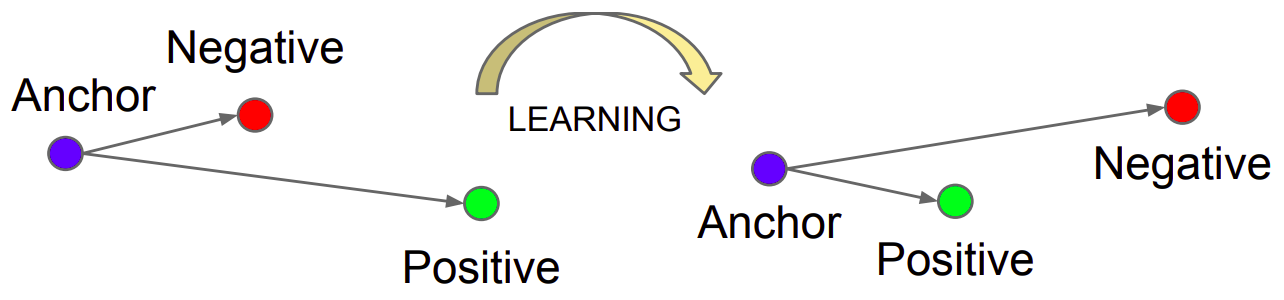
\includegraphics[width=\linewidth]{figures/triplet-ranking-loss}
    \caption[三元组排序损失函数训练示例图]{\textbf{三元组排序损失函数训练示例图。三元组排序损失函数最小化参照点(Anchor)与正样本点(Positive)的距离,最大化参照点(Anchor)与负样本点(Negative)的距离。来自~\cite{schroff2015facenet}。}}
    \label{fig:triplet-ranking-loss}
\end{figure*}

如图~\ref{fig:triplet-ranking-loss}所示,在训练过程中,三元组排序损失函数在最小化参照点与正样本点的距离的同时,最大化参照点与负样本点的距离,从而参照点更能区分正样本点和负样本点。与经典的三元组排序损失函数从训练样本中随机地选择负样本构建三元组不同,在训练的每个批次(batch),ITRL只选择最难区分的负样本(即与参照点距离最近的负样本)作为参照点的负样本点,因为最难的负样本会提供更多的具有区分性的信息,因此也更能区分距离较远的负样本,训练后的模型的性能也就更好。

对于本文研究即席视频检索问题,我们的目标是对于用户输入的查询句子,视频集的视频更加具有区分性,即与用户查询越相关的视频与查询的距离更近,相反,越不相关的视频与查询句子的距离更远。因此ITRL的参照点是查询句子,而正样本点是相关的视频而负样本点是不相关的视频。
对于一个给定的训练句子$s$,对应着一个与该句子相关的正样本视频$v^+$,和与该样本不相关的一系列视频$v^-$,因此ITRL的表达式如下公式~\ref{eq:itrl}所示:

\begin{equation}
    \label{eq:itrl}
    \left\{
        \begin{aligned}
            & v^{-*} & = & \mathop{\arg\max}_{v^- \in batch}(cms(s, v^-) - cms(s, v^+)), & \\
            & ITRL(s) & = & \max(0, \alpha + cms(s, v^{-*}) - cms(s, v^+)) &
        \end{aligned}
    \right.
\end{equation}
其中$\alpha$是超参数。

W2VV++模型:该模型将查询句子$s$和视频$v$都投影到一个公共的跨模态空间,并在该公共空间计算句子与视频的余弦相似度$cms(s,v)$,并根据该相似度在训练的每个批次如公式~\ref{eq:itrl}计算并优化损失函数$ITRL(s)$,即:
\begin{equation}
    \label{eq:loss-w2vv++}
    \begin{aligned}
        loss(s;\theta) = ITRL(s)
    \end{aligned}
\end{equation}
其中$\theta$为模型中的可学习参数。

SEA模型:该模型为每个句子编码器(bow,w2v,GRU)对查询句子$s$的编码向量构建一个独立的公共跨模态空间,并将视频$v$也分别投影到这些公共空间中,在每个公共空间中可以计算句子$s$与视频$v$的相似度,每对句子-视频对工产生3个相似度,即$cms_1(s,v)$,$cms_2(s,v)$和$csm_3(s,v)$,而该句子-视频对的相似度由这三个相似度的平均得到,即$cms(s,v):=\frac{1}{3}(cms_1(s,v)+cms_2(s,v)+cms_3(s,v))$。本文认为使用最终的句子-视频相似度来计算并优化ITRL函数对于多空间学习不是一种最优的做法,因为在一个训练批次里,根据最终的句子-视频相似度来选择最难负样本对于每个跨模态公共空间不是最有效的,而应该根据句子和视频在每个公共空间计算的相似度来选择句子$s$的最难负样本视频$v^{-*}$。因此,本文选择在每个公共空间计算$ITRL_i(s), i=1,2,3$,并且最终优化三个公共空间的联合目标函数,即:
\begin{equation}
    \label{eq:loss-sea}
    \begin{aligned}
        loss(s;\theta) = \sum_{i=1}^3 ITRL_i(s)
    \end{aligned}
\end{equation}
其中$\theta$为模型中的可学习参数。与平均融合每个空间的相似度类似,本文以相等的权重融合每个空间中计算的目标函数。如图\ref{fig:negative-examples}的所示,平均融合每个空间的目标函数在训练过程中产生更多样化的难样本,这样更加有利于模型的训练。

\begin{figure*}[tbh!]
    \centering
    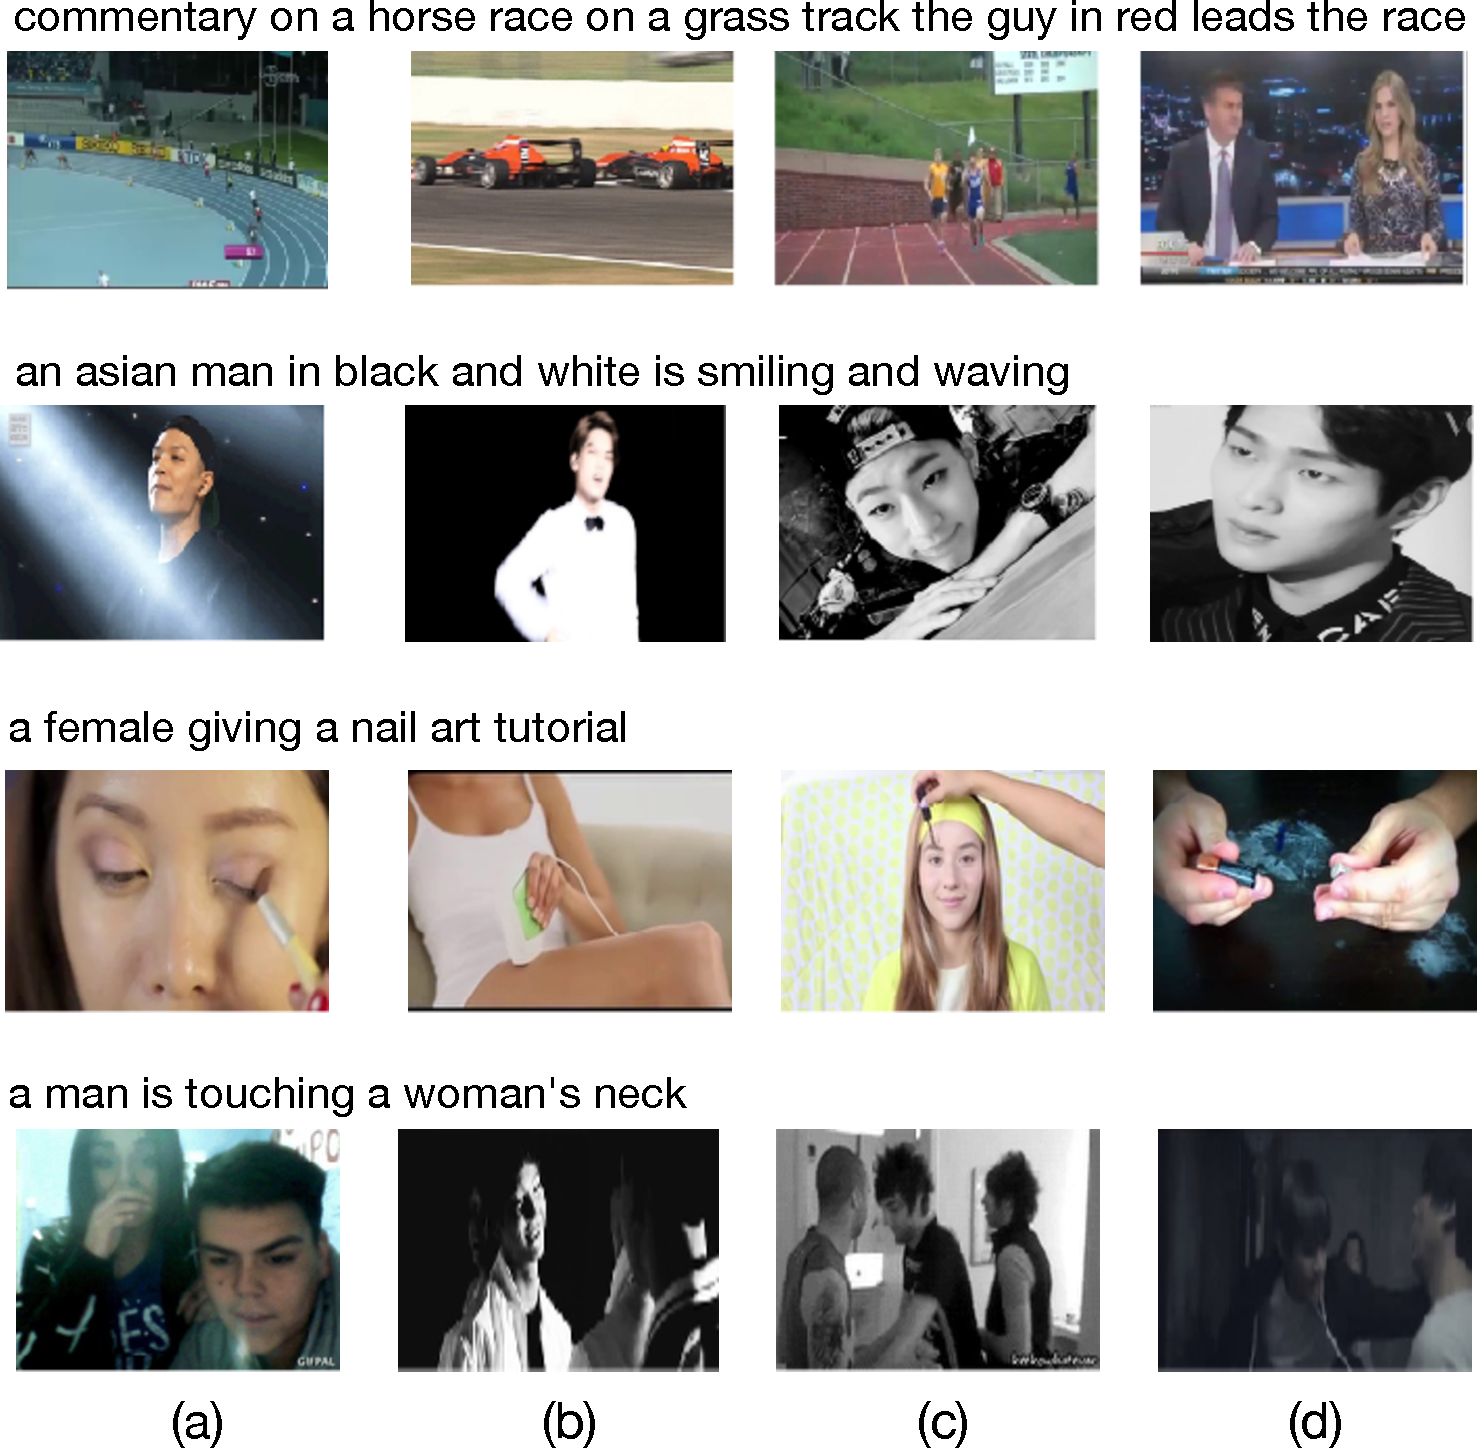
\includegraphics[width=\linewidth]{figures/single_vs_combined_loss}
    \caption[训练过程中对于特定的句子SEA模型自动选择的最难负样本视频的示例图]{\bfseries{训练过程中对于特定的句子SEA模型自动选择的最难负样本视频的示例图。第一列(a)根据先融合多空间的相似度再计算ITRL目标函数选择的最难负样本,而另外三列是根据为每个公共空间计算ITRL目标函数,而(b),(c),(d)分别为句子编码器$e_{bow}$,$e_{w2v}$和$e_{gru}$所投影的公共空间中选择的最难负样本。可见融合多空间的目标函数可以在每个批次产生更多样性的最难负样本。}}
    \label{fig:negative-examples}
\end{figure*}

\section{本章小结}
本章从句子编码网络、视频特征提取、转换网络和目标函数四个方面详细地介绍了本文研究的两个基于深度学习的即席视频检索算法W2VV++和SEA。W2VV++基于一个原本用于图像-句子相互检索的模型W2VV~\cite{dong2018predicting}进行了句子编码的改进,并在训练时使用更加有效的improved triplet ranking loss(ITRL)作为训练目标监督模型的训练,从而更好地适应于基于文本的视频检索任务。SEA模型在W2VV++的基础上采用多空间多目标函数的训练策略,即为每个句子编码器构建独立的公共跨模态空间,并且每个空间独立地使用ITRL作为目标函数监督各自空间的训练,最后句子与视频的相似度由句子与视频在所有公共空间计算的相似度取平均得到。

